\documentclass{beamer}

\usepackage{subfigure}
\usepackage{graphics}
\usepackage[margin=10pt,font=small,labelfont=bf, labelsep=endash, skip=0pt]{caption}

% Class options include: notes, notesonly, handout, trans,
%                        hidesubsections, shadesubsections,
%                        inrow, blue, red, grey, brown

% Theme for beamer presentation.
\usepackage{beamerthemesplit} 
% Other themes include: beamerthemebars, beamerthemelined, 
%                       beamerthemetree, beamerthemetreebars  

\title{Mahjong Solitaire}    % Enter your title between curly braces
\author{Sessa Carlos, Pizzagalli Lucas y Purita Nicol\'as}                 % Enter your name between curly braces
\institute{Instituto Tecnol\'ogico de Buenos Aires - ITBA}      % Enter your institute name between curly braces
\date{$20$ de Marzo del $2012$}                    % Enter the date or \today between curly braces

\begin{document}

% Creates title page of slide show using above information
\begin{frame}
  \titlepage
\end{frame}

\section{Juego}

\begin{frame}
  \frametitle{Juego}   % Insert frame title between curly braces

	El juego \textbf{Mahjong-Solitaire} consiste en eliminar todas las fichas de un tablero que posee 144 fichas. \\
	Las fichas deben ser removidas de a pares cumpliendo las condiciones de:
	
	\begin{itemize}
		\item No deben estar bloqueadas. (Figura \ref{fig:blocking})
		\item El par de ficha debe ser del mismo tipo.
	\end{itemize}		
	
\tiny{
\begin{table}
\begin{center}
	\begin{tabular}{|c|c|c|}
	\hline
	 Tipo de Ficha & Identificador & Cantidad\\
	\hline \hline
	\textit{Character} & 9 & 4 de c$\setminus$u \\
	\textit{Bamboo} & 9 & 4 de  c$\setminus$u  \\
	\textit{Circles} & 9 & 4 de  c$\setminus$u  \\
	\textit{Dragons} & 3 & 4 de  c$\setminus$u  \\	
	\textit{Winds} & 4 & 4 de  c$\setminus$u  \\
	\textit{Season} & 4 & 1 de c$\setminus$u \\
	\textit{Flowers} & 4 & 1 de  c$\setminus$u  \\
	\hline
	\end{tabular}
\end{center}
\caption{Distribuci\'on de fichas}
\label{tab:tiles}
\end{table}}
\end{frame}

\begin{frame}
\begin{figure}[hb]
  	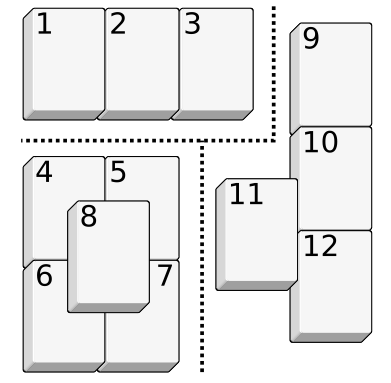
\includegraphics[scale=0.3]{../images/blocking.png}
	\caption{Ficha 2 es bloqueada por la 1 y 3. La ficha 4-7 est\'an bloqueadas por la 8. El resto de las fichas son movibles.}
  \label{fig:blocking}
\end{figure}
\end{frame}

\section{Desarrollo}

\begin{frame}
  \frametitle{Reglas}   % Insert frame title between curly braces
	La \textbf{Meta-Regla} existente en el problema es:
	\begin{itemize}
		\item Tomar un par de fichas y removerlas mientras cumpla las condiciones mencionadas.
	\end{itemize}
\end{frame}

\begin{frame}
  	\frametitle{Funci\'on de Costo}   % Insert frame title between curly braces
	Dado que el objetivo del juego es simplemente retirar todas las fichas del tablero, y las mismas deben ser retiradas siempre de a pares, la funci\'on de costo propuesta es constante, haciendo referencia a la remoci\'on de un par del tablero. Dicha funci\'on se denomina \textit{$g_1$}. \\
\end{frame}

\section{Heur\'isticas}
\begin{frame}
  \frametitle{Heur\'isticas}
   \begin{itemize}
	   	\item \textbf{\textit{Pair:}} Todo par de fichas con posibilidad de ser retiradas del tablero en un estado determinado.
	   	\item \textbf{\textit{Payers:}} Lista de \textit{Pares}. \\
   \end{itemize}
   Las heur\'isticas son:
   \begin{itemize}
		\item \textbf{M\'as Alta} \textit{(h1)}.
		\item \textbf{Mayor cantidad de fichas horizontales} \textit{(h2)}.
		\item \textbf{Generador M\'aximo de \textit{Payers}} \textit{(h3)}.
	\end{itemize}
\end{frame}

\begin{frame}
\frametitle{M\'as Alta \textit{(h1)}}
Se libera el \textit{Pair} de m\'as alto nivel. En el mejor de los casos la remoci\'on de una ficha en una capa m\'as alta puede liberar cuatro fichas, lo cual aumenta la cantidad de \textbf{Payers} en la siguiente jugada.
\end{frame}

\begin{frame}
\frametitle{Mayor cantidad de fichas horizontales \textit{(h2)}}
Esta heur\'istica busca reducir la posibilidad de eliminar una fila del tabler. La heur\'istica se basa en calcular la cantidad de fichas que posee cada fila en la que se encuentran cada ficha que compone el \textit{Pair} , esto se calcula como:
			\begin{eqnarray}
				X_{1}  & = & \# Fichas_{Fila de F_{1}} \\
				X_{2}  & = & \# Fichas_{Fila de F_{2}} \\
				\textbf{h2} & = & \#(FichasTotales - ( X_{1} + X_{2} )) / 2
			\end{eqnarray}
		donde $F_{1}$ y $F_{2}$ son las fichas que componen el \textit{Pair}. 
\end{frame}

\begin{frame}
\frametitle{Generador M\'aximo de \textit{Payers} \textit{(h3)}}

Esta heur\'isitca se basa en eliminar los \textit{Pairs} que generen mayor cantidad de \textit{Payers} en el pr\'oximo estado.
\end{frame}

\section{Resultados}

\begin{frame}
\frametitle{Tablero Layout1}
\begin{figure}[hb]
	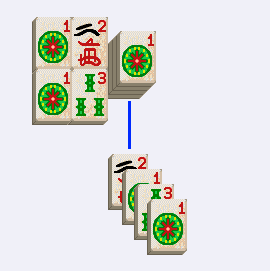
\includegraphics[scale=0.3]{../Boards/Layout1.png}
\end{figure}
\end{frame}

\begin{frame}
\frametitle{Layout1}

\tiny{
\begin{table}[h]
\begin{center}
	\begin{tabular}{|p{1.3cm}|p{1.0cm}|p{1cm}|p{1cm}|p{1cm}|p{1cm}|p{2cm}|}
	\hline
	 Algoritmo & Heur\'istica & Nodos expandidos & Nodos en la frontera & Nodos generados & Profundidad de la Soluci\'on & Tiempo de Procesamiento\\
	\hline \hline
		 \multicolumn{6}{|c|}{Layout 1} \\
	\hline
	\textit{DFS} & - & 6 & 0 & 6 & 4 & 32ms \\
	\textit{BFS} & - & 7 & 0 & 6 & 4 & 10ms \\
	\textit{Produndizaci\'on Iterativa} & - & 7 &  7 & 19 & 4 & 12ms \\
	\textit{$A^*$} & h1 & 4 & 2 & 5 & 4 & 14ms \\
	\textit{$A^*$} & h2 & 4 & 2 & 5 & 4 & 14ms \\
	\textit{$A^*$} & h3 & 4 & 2 & 5 & 4 & 14ms \\
	\hline
	\end{tabular}
\end{center}
\label{tab:costLayout1}
\end{table}}

\end{frame}

\begin{frame}
\frametitle{Tablero Layout2}
\begin{figure}[hb]
	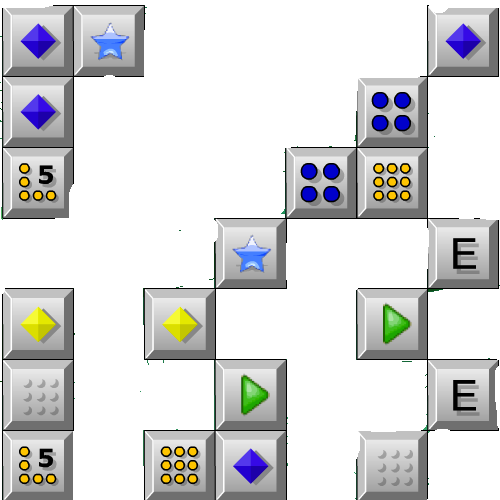
\includegraphics[scale=0.3]{../Boards/Layout3.png}
	 \label{fig:layout3}
\end{figure}
\end{frame}

\begin{frame}
\frametitle{Layout2}

\tiny{
\begin{table}[h]
\begin{center}
	\begin{tabular}{|p{1.3cm}|p{1.0cm}|p{1cm}|p{1cm}|p{1cm}|p{1cm}|p{2cm}|}
	\hline
	 Algoritmo & Heur\'istica & Nodos expandidos & Nodos en la frontera & Nodos generados & Profundidad de la Soluci\'on & Tiempo de Procesamiento\\
	\hline \hline
		 \multicolumn{6}{|c|}{Layout 2} \\
	\hline
	\textit{DFS} & - &  11 & 57 & 10 & 10 & 74ms \\
	\textit{BFS} & - & 5944 & 34491 & 5944 & ? & 5' \\
	\textit{Produndizaci\'on Iterativa} &  - & 7550 & 33571 & 5696 & ? & 5' \\	
	\textit{$A^*$} & h1 & 10 & 57 & 11 & 10 & 130ms \\
	\textit{$A^*$} & h2 & 10 & 57 & 11 & 10 & 97ms \\
	\textit{$A^*$} & h3 & 5983 & 34934 & 5983 & ? & 5'\\
	\hline
	\end{tabular}
\end{center}
\label{tab:costLayout3}
\end{table}}

\end{frame}

\begin{frame}
\frametitle{Tablero Layout3}
\begin{figure}[hb]
	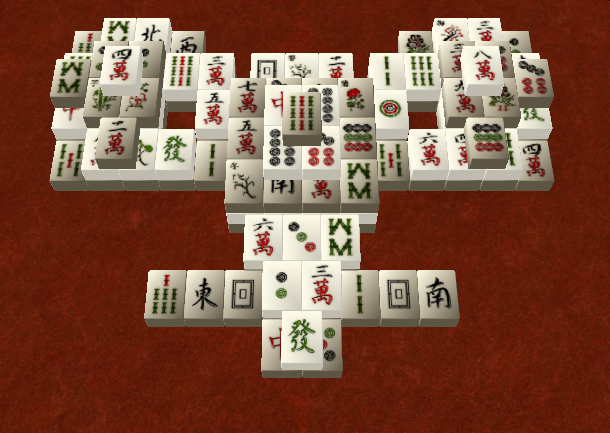
\includegraphics[scale=0.3]{../Boards/Layout4.png}
	 \label{fig:layout4}
\end{figure}
\end{frame}

\begin{frame}
\frametitle{Layout3}

\tiny{
\begin{table}[h]
\begin{center}
	\begin{tabular}{|p{1.3cm}|p{1.0cm}|p{1cm}|p{1cm}|p{1cm}|p{1cm}|p{2cm}|}
	\hline
	 Algoritmo & Heur\'istica & Nodos expandidos & Nodos en la frontera & Nodos generados & Profundidad de la Soluci\'on & Tiempo de Procesamiento\\
	\hline \hline
		 \multicolumn{6}{|c|}{Layout 3} \\
	\hline
	\textit{DFS} & - & 73 & 1438 & 72 & 72 & 2' 708ms \\
	\textit{BFS} & - & 641 & 15705 & 641 & ? & 5' \\
	\textit{Produndizaci\'on Iterativa} & - & 620 & 14964 & 587 & ? & 5' \\	
	\textit{$A^*$} & h1 & 525 &  10660 & 525 & ? & 5' \\
	\textit{$A^*$} & h2 & 72 & 1438 & 73 & 72 & 2'' 864ms\\
	\textit{$A^*$} & h3 & 349 & 17903 & 349 & ? & 5' \\	
	\hline
	\end{tabular}
\end{center}
\label{tab:costLayout4}
\end{table}}

\end{frame}

\begin{frame}
\textbf{\Huge{Preguntas?}}
\end{frame}

\end{document}
